% Created 2016-08-17 Wed 14:38
\documentclass[tikz]{standalone}

\usepackage[utf8]{inputenc}
\usepackage[T1]{fontenc}
\usepackage{helvet}
\usepackage{../../templates/msc}

\renewcommand{\familydefault}{\sfdefault}

\tikzset{
every picture/.style={
line width=1pt
}}

\usepackage{tikz}
\author{Holger Karl}
\date{\today}
\title{}


\begin{document}
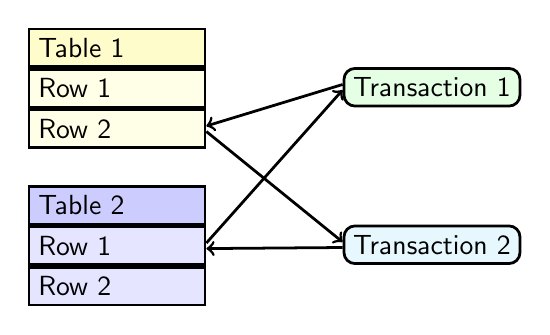
\begin{tikzpicture}

  \node (t2) [fill=blue!20, draw, align=left, text width = 2cm] {Table 2};
  \node (t2r1) [fill=blue!10, draw, align=left, below right, text  width = 2cm] at (t2.south west)  {Row  1};
  \node (t2r2) [fill=blue!10, draw, align=left, below right, text  width = 2cm] at (t2r1.south west) {Row 2};

  \node (t1) [fill=yellow!20, draw, align=left, text width = 2cm] at (0, 2) {Table 1};
  \node (t1r1) [fill=yellow!10, draw, align=left, below right, text  width = 2cm] at (t1.south west)  {Row  1};
  \node (t1r2) [fill=yellow!10, draw, align=left, below right, text  width = 2cm] at (t1r1.south west) {Row 2};

  \node (tr1) [draw, rounded corners, fill=green!10] at (4,1.5)  {Transaction 1};
  \node (tr2) [draw, rounded corners, fill=cyan!10] at (4,-0.5)  {Transaction 2};

  \draw [->] ([yshift=+1pt]t2r1.east) -- ([yshift=-1pt]tr1.west); 
  \draw [<-] ([yshift=+1pt]t1r2.east) -- ([yshift=1pt]tr1.west); 
   
  \draw [<-] ([yshift=-1pt]t2r1.east) -- ([yshift=-1pt]tr2.west); 
  \draw [->] ([yshift=-1pt]t1r2.east) -- ([yshift=+1pt]tr2.west); 

\end{tikzpicture}
\end{document}